%% Copernicus Publications Manuscript Preparation Template for LaTeX Submissions
%% ---------------------------------
%% This template should be used for copernicus.cls
%% The class file and some style files are bundled in the Copernicus Latex Package, which can be downloaded from the different journal webpages.
%% For further assistance please contact Copernicus Publications at: production@copernicus.org
%% https://publications.copernicus.org/for_authors/manuscript_preparation.html


%% Please use the following documentclass and journal abbreviations for discussion papers and final revised papers.

%% 2-column papers and discussion papers
\documentclass[bg, manuscript]{copernicus}



%% Journal abbreviations (please use the same for discussion papers and final revised papers)


% Advances in Geosciences (adgeo)
% Advances in Radio Science (ars)
% Advances in Science and Research (asr)
% Advances in Statistical Climatology, Meteorology and Oceanography (ascmo)
% Annales Geophysicae (angeo)
% Archives Animal Breeding (aab)
% ASTRA Proceedings (ap)
% Atmospheric Chemistry and Physics (acp)
% Atmospheric Measurement Techniques (amt)
% Biogeosciences (bg)
% Climate of the Past (cp)
% DEUQUA Special Publications (deuquasp)
% Drinking Water Engineering and Science (dwes)
% Earth Surface Dynamics (esurf)
% Earth System Dynamics (esd)
% Earth System Science Data (essd)
% E&G Quaternary Science Journal (egqsj)
% European Journal of Mineralogy (ejm)
% Fossil Record (fr)
% Geochronology (gchron)
% Geographica Helvetica (gh)
% Geoscience Communication (gc)
% Geoscientific Instrumentation, Methods and Data Systems (gi)
% Geoscientific Model Development (gmd)
% History of Geo- and Space Sciences (hgss)
% Hydrology and Earth System Sciences (hess)
% Journal of Micropalaeontology (jm)
% Journal of Sensors and Sensor Systems (jsss)
% Mechanical Sciences (ms)
% Natural Hazards and Earth System Sciences (nhess)
% Nonlinear Processes in Geophysics (npg)
% Ocean Science (os)
% Primate Biology (pb)
% Proceedings of the International Association of Hydrological Sciences (piahs)
% Scientific Drilling (sd)
% SOIL (soil)
% Solid Earth (se)
% The Cryosphere (tc)
% Weather and Climate Dynamics (wcd)
% Web Ecology (we)
% Wind Energy Science (wes)


%% \usepackage commands included in the copernicus.cls:
%\usepackage[german, english]{babel}
%\usepackage{tabularx}
%\usepackage{cancel}
%\usepackage{multirow}
%\usepackage{supertabular}
%\usepackage{algorithmic}
%\usepackage{algorithm}
%\usepackage{amsthm}
%\usepackage{float}
%\usepackage{subfig}
%\usepackage{rotating}


\begin{document}

\title{Causes and implications of vegetation distribution biases in UKESM}


% \Author[affil]{given_name}{surname}

\Author[1]{Douglas I}{Kelley}
\Author[2]{Eddy}{Robertson}
\Author[2Burke]{Eleanor}{Burke}
\Author[2]{Chantelle}{Burton}
\Author[1]{Phil}{Harris}
\Author[3]{Rebecca}{Varney}
\Author[3]{Rob}{King}
\Author[4]{Nic}{Gendey}
\Author[5, 6]{Rob}{Parker}
\Author[2]{Debbie}{Hemming}
\Author[1]{Rachael}{Turton}
\Author[7,8]{Colin}{Jones}

% Other people who have done a butt load of JULES-ES work that should be included.
% Please add names :D
\Author[1]{Rich}{Ellis}
\Author[2]{Spencer}{Liddicoat}
\Author[2, 3]{Karina}{Williams}
\Author[2]{Alistair}{Sellar}
\Author[2]{Andy}{Whilshire}
\Author[1]{Chris}{Jones}
\Author[3]{Anna}{Harper}

\affil[1]{UK Centre for Ecology and Hydrology, Wallingford, OX10 8BB, UK}
\affil[2]{Met Office Hadley Centre, Exeter, EX1 3PB, UK}
\affil[3]{College of Life and Environmental Science, University of Exeter, Exeter, EX4 4SB, UK}
\affil[4]{Met Office, Wallingford, OX10 8BB, UK}
\affil[5]{National Centre for Earth Observation, Leicester, UK}
\affil[6]{Earth Observation Science, School of Physics and Astronomy, University of Leicester, Leicester, UK}
\affil[7]{National Centre for Atmospheric Science, UK}
\affil[8]{School of Earth and Environment, University of Leeds, Leeds, UK}

%% The [] brackets identify the author with the corresponding affiliation. 1, 2, 3, etc. should be inserted.

%% If an author is deceased, please add a further affiliation and mark the respective author name(s) with a dagger, e.g. "\Author[2,$\dag$]{Anton}{Aman}" with the affiliations "\affil[2]{University of ...}" and "\affil[$\dag$]{deceased, 1 July 2019}"


\correspondence{Douglas I Kelley (doukel@ceh.ac.uk)}

\runningtitle{UKESM vegetation distribution biases}

\runningauthor{Douglas I Kelley}





\received{}
\pubdiscuss{} %% only important for two-stage journals
\revised{}
\accepted{}
\published{}

%% These dates will be inserted by Copernicus Publications during the typesetting process.


\firstpage{1}

\maketitle



\begin{abstract}
Aim:
\citep{Sellar2019-bo}

\end{abstract}


\copyrightstatement{TEXT}


\introduction  %% \introduction[modified heading if necessary]
TEXT


\section{Model overview}
TEXT

\subsection{UKESM and atmosphere stuff}

\subsection{JULES overview}

\subsubsection{Veg Dynamics}

\subsubsection{Land use}

\subsubsection{Phenology}

\subsubsection{Carbon/photosynthesis}

\subsubsection{Nitrogen}

\subsubsection{Cold stuff}

\subsubsection{Veg snow interactions}

\section{}

\subsection{Evaluation methods}

We use the International Land Model Benchmarking (ILAMB) tool (Collier et al., 2018) here to evaluate model performance across multiple variables compared to observations. ILAMB was designed to provide a quantitative assessment of model fidelity across a wide range of terrestrial biogeochemical processes and interactions with hydrology and climate, within several key categories: the ecosystem and carbon cycle, hydrological cycle, radiation and energy, and forcings. The tool uses remote sensing, reanalysis data and fluxnet site measurements to benchmark performance and produce statistical scores of model results. 

We also use Kelley et al. (2013)

\subsubsection{Annual average}
The sum the squared (for $NMSE$) or absolute (for $NME$) distance between observations ($obs$) and reconstructed burnt  rea from an ensemble member (sim()) over all cells  ( ) weighted by cell area ( ) and normalised by mean variation in obs

\begin{equation}
    NME = \frac{\Sigma_i A_i \times  |sim - obs_i |}{\Sigma_i A_i \times |\bar{obs} - obs_i |} \  \text{   and   } \
    NMSE = \frac{\Sigma_i A_i \times  (sim- obs_i) }{\Sigma_i A_i \times (\bar{obs} - obs_i )}
\end{equation}

\subsubsection{Seasonal}
Seasonality comparisons are conducted in three parts as  (Kelley et al., submitted, 2013a): 1)modality - i.e how many “seasons” there are in a given year; 2), phase, or timing, of the season; and 3) seasonal concentration (inverse season length).

To determine the modality of a given cell, we first calculated the monthly climatology. The month of the minimum burnt area from this climatology is defined as the start of the “fire year”. We then find the position of each maxima turning point throughout the year:	
\begin{equation}

    P = \left\{p_i | \frac{dv(p_i)}{dt} = 0 \wedge \frac{d^2v(p_i)}{dt^2} < 0 \wedge v(p_i) < v(p_{i+1}) \right\}

\end{equation}

where $v(1) = min(v)$

The modality (MOD) is the prominence of each of these turning points (i.e the minimum drop required to the next turning point), weighted by the distance to the next turning point. This is normalised by the height of the month of maximum burnt area

\begin{equation}
    MOD =1 + \frac{ \Sigma_{i-1} \big( V(p_i) - min\left\{ v(p_i), v(p_{i+1}) \right\} \big) \times \big( 1 - cos(\theta) \big)}{2 \times \big(max(v) - v(1) \big)}
\end{equation}

If there are no turning points, then modality is set to 0. If there is one turning point, MOD is 1. The higher the number beyond that, the higher the modality. Observational and simulated MOD  was then compared using NME/NMSE.

For phase and concentration, each month, m, can be represented by a vector in the complex plane whose direction (m) corresponds to the time of year and length to the magnitude of the variable for that month:
\begin{equation}
    \theta_m = 2 \times \pi \times (m-1) / 12
\end{equation}

A mean vector L can be calculated by averaging the real (Lx) and imaginary (Ly) parts of the 12 vectors (xm).

\begin{equation}
    L_x = \Sigma_m x_m \times cos(\theta_m) \ \text{   and   } \
    L_y = \Sigma_m x_m \times sin(\theta_m)
\end{equation}

Seasonal concentration (C) is the mean vector length by the annual average of the given variable, whilst seasonal phase (P) is the direction of the vector:

\begin{equation}
    C = \frac{\sqrt{L_x^2 + L_y^2}}{\Sigma_m x_m}
\end{equation}

\begin{equation}
    P arctan{L_x/L_y}
\end{equation}

C is equal to 1 when a give variable is concentrated into one month, whilse P corresponds to that month. concentration is zero and phase is undefined if the variable  is evenly spread throughout the year, and the is not included in subsequent phase comparisons. Cis compared using NME/NMSE step 1. Phase is compared using mean phase difference (MPD), which represents the average timing erro, as a proportion of the maximum phase mismatch of 6 months.

\begin{equation}
    MPD = \pi^{-1} \times \Sigma_m A_i \times arccos \big[ cos \big(P_{sim, i} - P_{obs, i} \big) \big] / \Sigma_i A_i 
\end{equation}

\subsubsection{Metric interpretation}
Smaller NME, NMSE and MPD scores indicate a better agreement between simulation and observation, with a perfect score (i.e., simulation that perfectly matches observations) of 0. We also used three null models to help interpret the score as per (Burton et al., 2019; Kelley et al., 2019). The mean null model compares the mean of all observations with the observations. For NME and NMSE, the mean null model is always 1 as these metrics are normalised by the mean difference.. The best “single value” model for NME and MM compares the median of observations to observations. By definition, it’s score is less than or equal to the mean model score. The mean and median null model scores for MPD depends on the observations. The “randomly resampled” null model compares randomly-resampled observations (without replacement) to the observations. The score depends on resampling order, so we used 1000 bootstraps to determine the null models distribution. 

\subsection{Benchmark datasets}

\subsubsection{Climate}
Here we estimate the functional response of GPP to precipitation and surface downward shortwave radiation (SWR). For the global analysis, we use total grid points binned in terms of the independent variable (x) using 25 bins. In each bin, we compute the mean value of the corresponding dependent variable (y) to approximate the functional dependence of y on x. Data points show the mean and the error bars reflect the standard deviation range. We then assess the relationships by region using a simple scatter plot, first for South America tropical forest, and then South East Asia. Model data in all cases is the mean of the 9 ensemble members evaluated against observations from GBAF (GPP), CERES (SWR), and GPCP2 (precipitation) for 1982-2008 mean (see plots in section entitled “Climate Relationships”).

\subsubsection{Vegetation cover}

\subsubsection{LAI}

\subsubsection{Carbon (inc. Turnover)}

\subsubsection{Wetland}
We process the UKESM Historical ensemble members from 2000 - 2014 and calculate the ensemble mean, regridded to 0.5 x 0.5 degrees.

The SWAMPS-GLWD dataset (Poulter et al., 2017) is a 0.5 x 0.5 degree global wetland dynamic dataset that integrates the static Global Lakes and Wetlands Dataset (Lehner and Döll, 2004)with observations of the inundation seasonal cycle from the Surface WAter Microwave Product Series (Schroeder et al., 2015). SWAMPS-GLWD covers 2000 - 2018, overlapping with the UKESM historical up to 2014.

We compare the UKESM wetland fraction (fracWet) to the wetland fraction obtained from SWAMPS-GLWD. We calculate the zonal mean of both data sets between 2000 - 2014, as well as calculating the variability (standard deviation) in the temporal domain.

\subsubsection{River flow}
Modelled, long-term, annual river flow is compared against observations (Dai et al., 2009). For the direct comparison we use the Dai et al, 2009 dataset from 925 stations which only uses observations and does not infill using land surface model output. Only 1990-2005 mean annual river flow is assessed, because at the sub-annual time-scale some river flow measurements will be impacted by the presence of dams upstream, and dams are not yet parameterised in UKESM1. We only make comparisons with the observations where the time series overlap, which results in a comparison against 134 stations. There is a strong correlation with the multi-annual river flow (figure ***) and obtain a correlation coefficient between modelled and observed  for the multi-annual mean and  log of river flow are 0.96 and 0.84 respectively. If we compare this to a similar off-line run where JULES is forced with observations we obtain correlation coefficients of 0.97 and 0.85 respectively, indicating that on a multi-year time scale UKESM is reproducing river flow well overall across the globe.

\section{results}

\subsection{Vegetation Distribution}
\begin{itemize}
    \item A lack on mix of tree and herb cover in much of the world, particularly Australia, Africa, Temperate America. The same could be true for Boreal regions, though there is disagreement in the observations here.
    \item Australia and SE Asia also show to tight a transition from non-vegetated to vegetated (R2 triangle figure)
    \item causes too much tree cover extent and, in some places, to much bare ground with very rapid transitions.
    \item grass extent is generally to small, but where grass does occur, there is too much of it.
    \item Too much bare soil in SE Asia, North Africa, possibly in Australia though depending on observations
    \item Too extensive in South Africa, North Africa, Boreal America, SE Asia, 
\end{itemize}


\begin{figure*}[t]
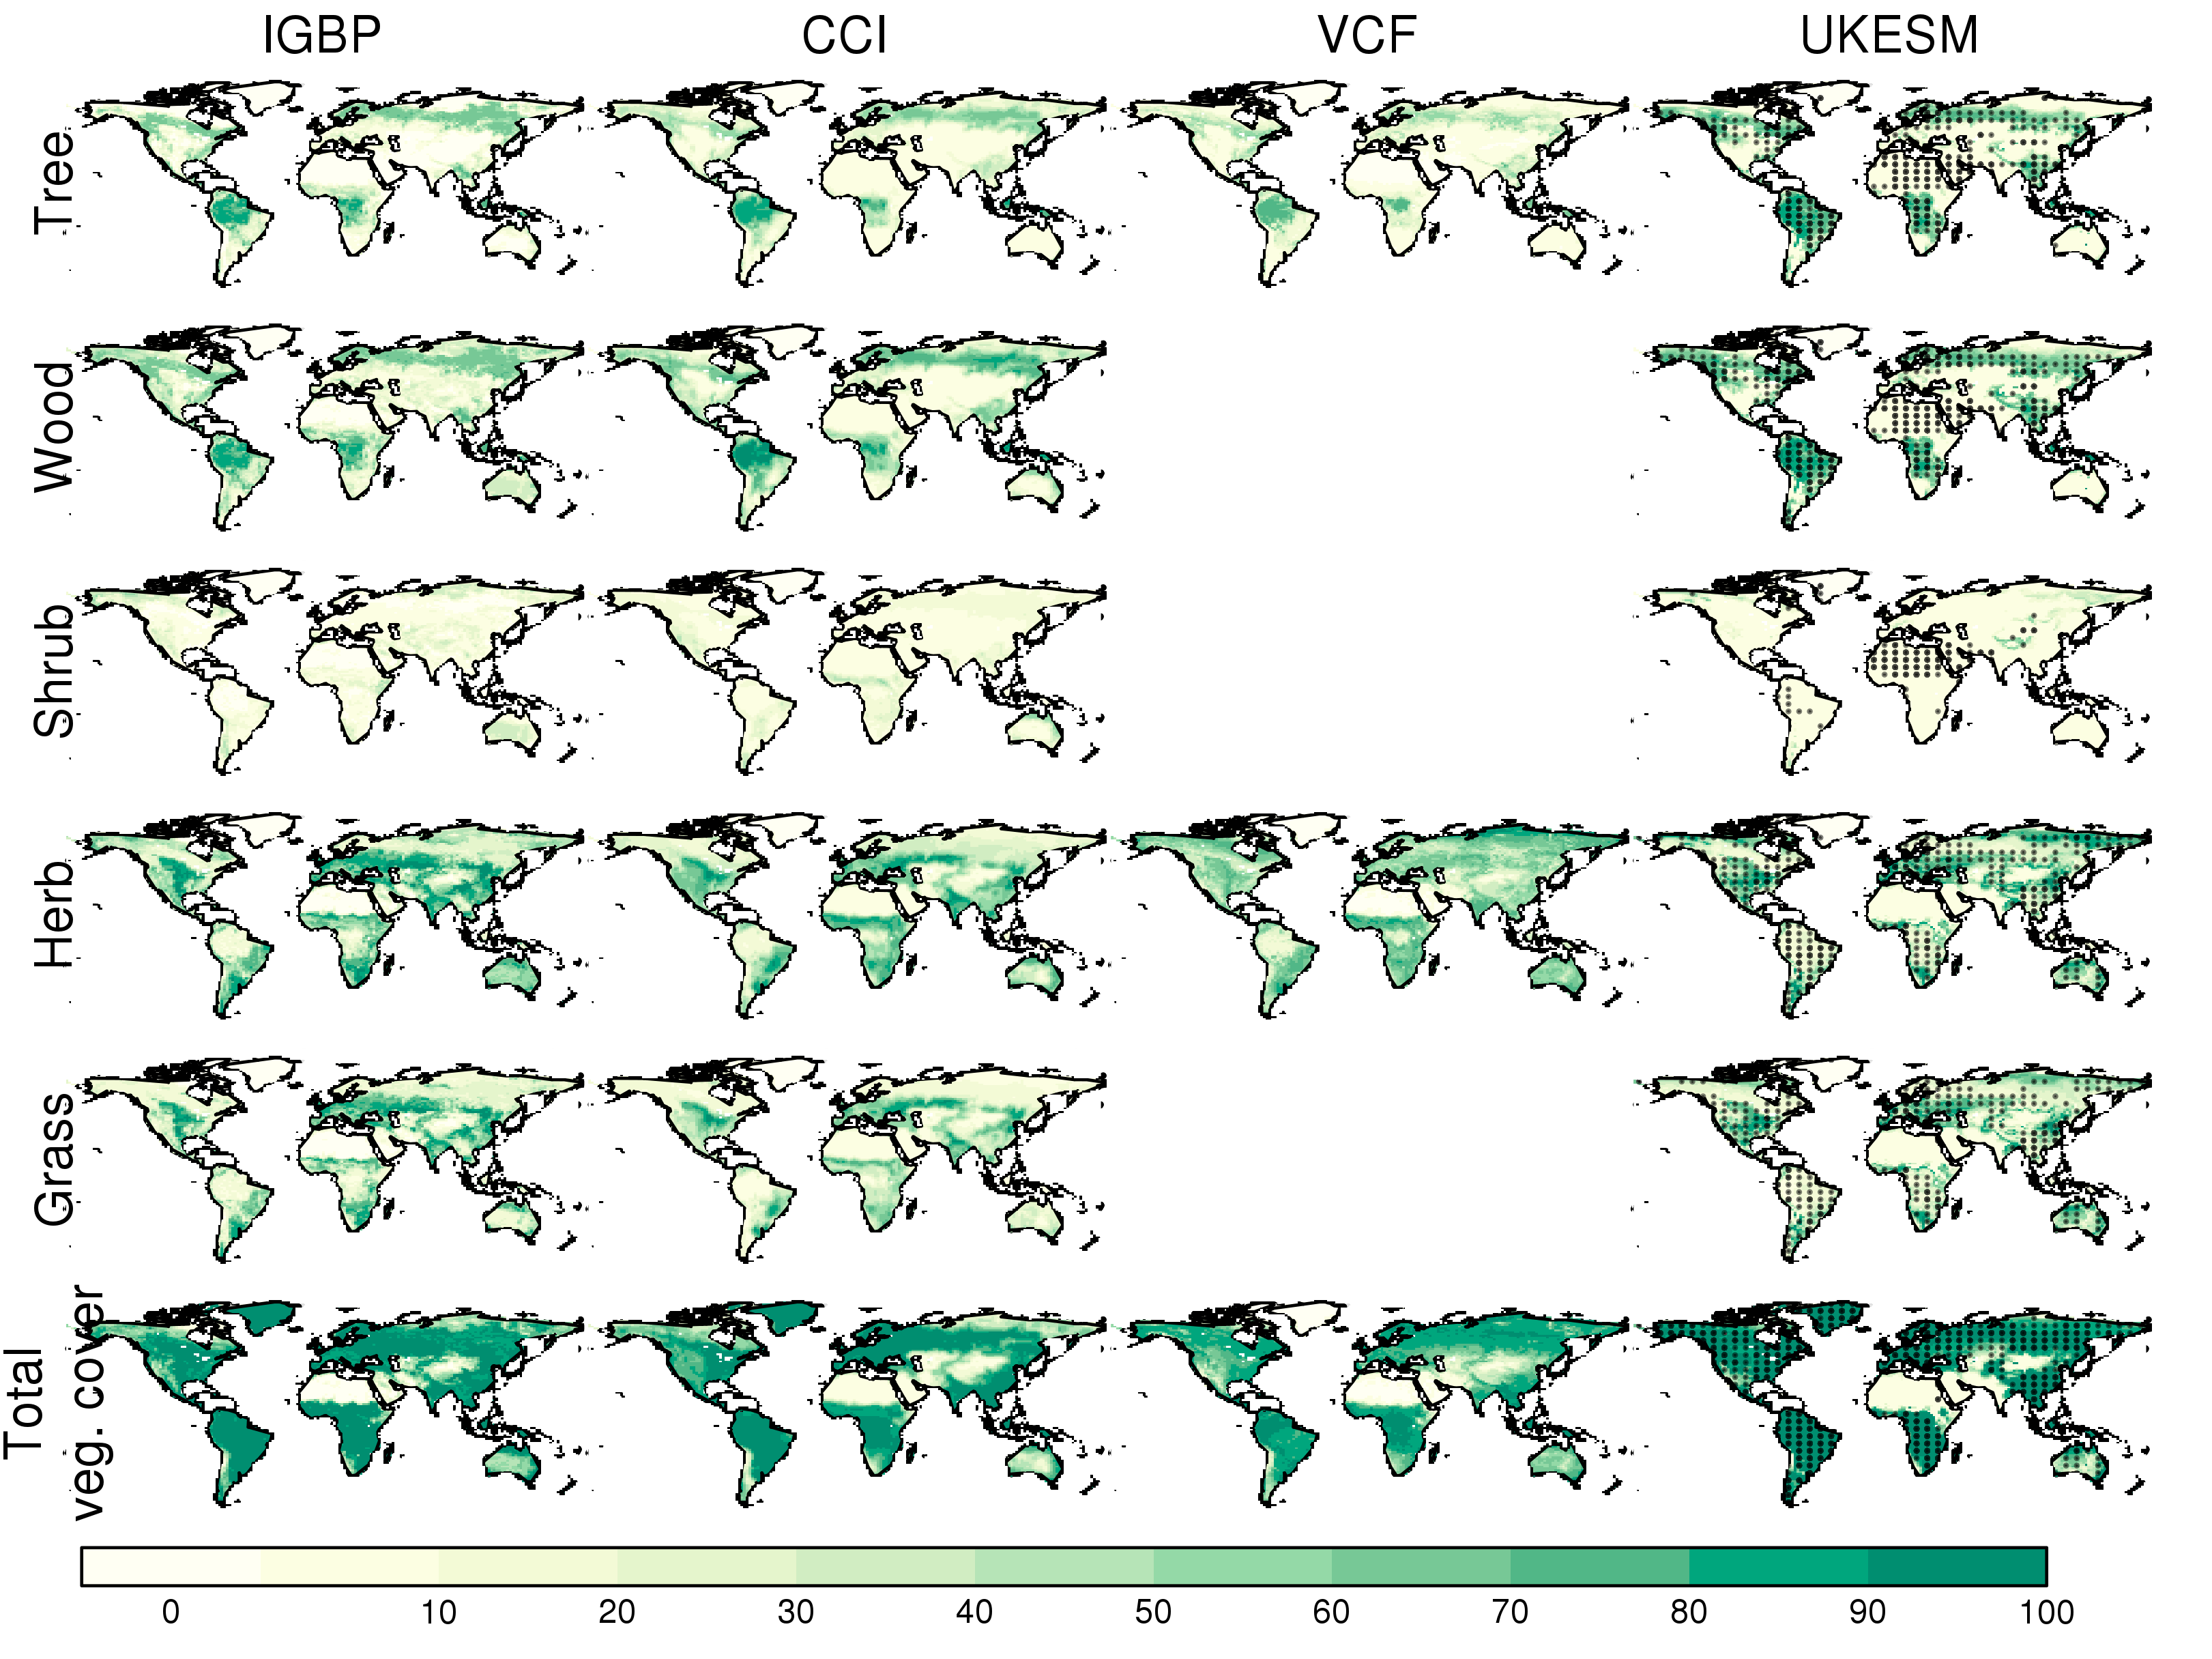
\includegraphics[width=12cm]{figs/vegDist.png}
\caption{Observed vs simulated percentage vegetation cover. From top to bottom: Tree, wood, shrub, herb, grass and total vegetative cover. From left to right, IGBP <<ref>>, CCI <<ref>>, VCF <<ref>> observations and simulated by UKESM. Dots in the UKESM column show variation in ensemble members}
\end{figure*}

\subsection{Lack of process representation}

\subsubsection{Fire}

\begin{figure}[t]
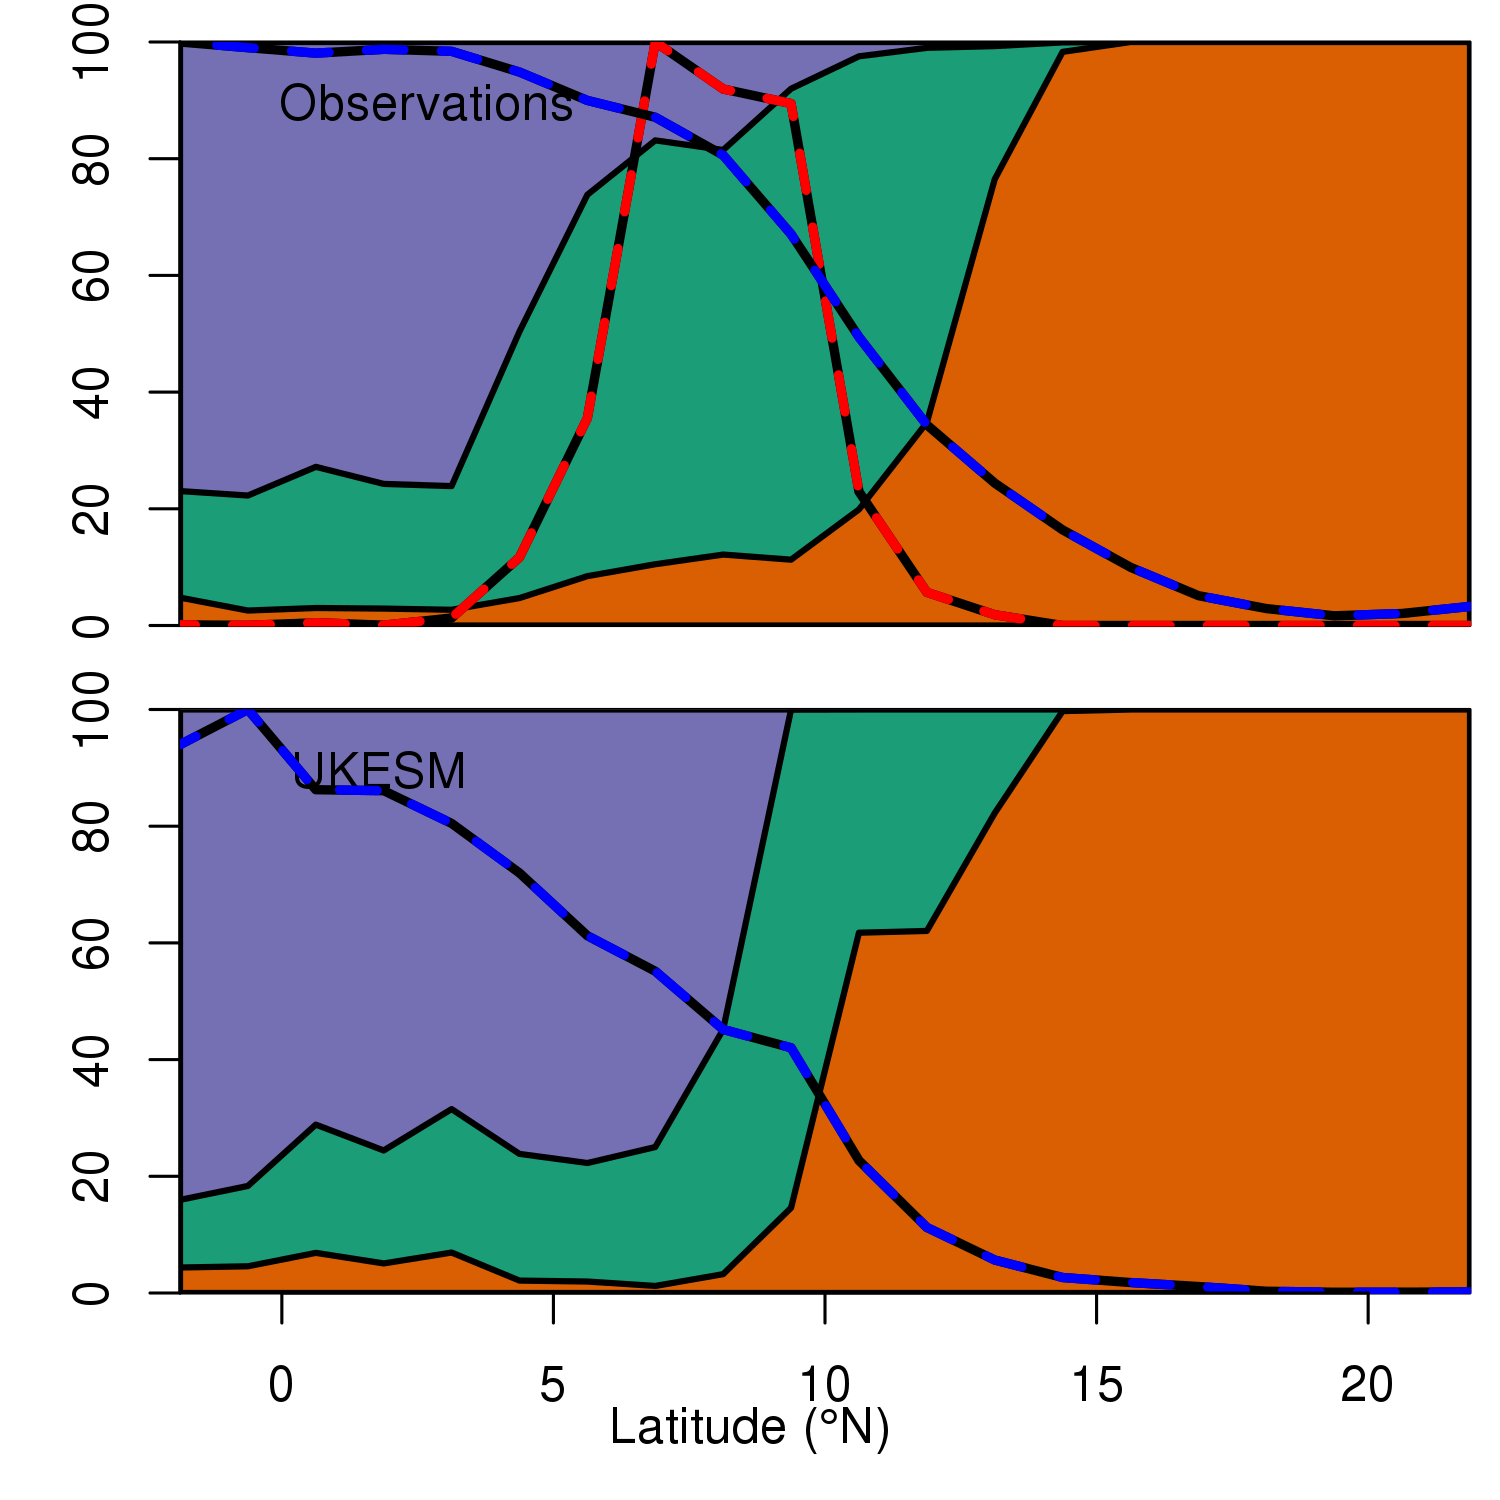
\includegraphics[width=8.3cm]{figs/trasect_AFRICA.png}
\caption{Transect of vegetation distribution from VCF observations and UKESM ensemble member u-bc179 along the longitude line of xx, spanning central Congo to central Sahara. Purple represents distribution of trees, green grasses and orange bare ground. Blue dotted line is observed mean annual precipitation from CRUTS 4.01 and u-bc179. Red dotted line is observed annual burnt area from GFED4s}
\end{figure}

\subsubsection{soils}



% something from Eleanor, Karina

\conclusions  %% \conclusions[modified heading if necessary]
TEXT

%% The following commands are for the statements about the availability of data sets and/or software code corresponding to the manuscript.
%% It is strongly recommended to make use of these sections in case data sets and/or software code have been part of your research the article is based on.

\codeavailability{TEXT} %% use this section when having only software code available


\dataavailability{TEXT} %% use this section when having only data sets available


\codedataavailability{TEXT} %% use this section when having data sets and software code available


\sampleavailability{TEXT} %% use this section when having geoscientific samples available


\videosupplement{TEXT} %% use this section when having video supplements available


\appendix
\section{}    %% Appendix A

\subsection{}     %% Appendix A1, A2, etc.


\noappendix       %% use this to mark the end of the appendix section

%% Regarding figures and tables in appendices, the following two options are possible depending on your general handling of figures and tables in the manuscript environment:

%% Option 1: If you sorted all figures and tables into the sections of the text, please also sort the appendix figures and appendix tables into the respective appendix sections.
%% They will be correctly named automatically.

%% Option 2: If you put all figures after the reference list, please insert appendix tables and figures after the normal tables and figures.
%% To rename them correctly to A1, A2, etc., please add the following commands in front of them:

\appendixfigures  %% needs to be added in front of appendix figures

\appendixtables   %% needs to be added in front of appendix tables

%% Please add \clearpage between each table and/or figure. Further guidelines on figures and tables can be found below.



\authorcontribution{TEXT} %% this section is mandatory

\competinginterests{TEXT} %% this section is mandatory even if you declare that no competing interests are present

\disclaimer{TEXT} %% optional section

\begin{acknowledgements}
TEXT
\end{acknowledgements}




%% REFERENCES

%% The reference list is compiled as follows:

%\begin{thebibliography}{}
%
%\bibitem[AUTHOR(YEAR)]{LABEL1}
%REFERENCE 1

%\bibitem[AUTHOR(YEAR)]{LABEL2}
%REFERENCE 2
%
%\end{thebibliography}

%% Since the Copernicus LaTeX package includes the BibTeX style file copernicus.bst,
%% authors experienced with BibTeX only have to include the following two lines:
%%
\bibliographystyle{copernicus}
\bibliography{References.bib}
%%
%% URLs and DOIs can be entered in your BibTeX file as:
%%
%% URL = {http://www.xyz.org/~jones/idx_g.htm}
%% DOI = {10.5194/xyz}


%% LITERATURE CITATIONS
%%
%% command                        & example result
%% \citet{jones90}|               & Jones et al. (1990)
%% \citep{jones90}|               & (Jones et al., 1990)
%% \citep{jones90,jones93}|       & (Jones et al., 1990, 1993)
%% \citep[p.~32]{jones90}|        & (Jones et al., 1990, p.~32)
%% \citep[e.g.,][]{jones90}|      & (e.g., Jones et al., 1990)
%% \citep[e.g.,][p.~32]{jones90}| & (e.g., Jones et al., 1990, p.~32)
%% \citeauthor{jones90}|          & Jones et al.
%% \citeyear{jones90}|            & 1990



%% FIGURES

%% When figures and tables are placed at the end of the MS (article in one-column style), please add \clearpage
%% between bibliography and first table and/or figure as well as between each table and/or figure.


%% ONE-COLUMN FIGURES

%%f
%\begin{figure}[t]
%\includegraphics[width=8.3cm]{FILE NAME}
%\caption{TEXT}
%\end{figure}
%
%%% TWO-COLUMN FIGURES
%
%%f
%\begin{figure*}[t]
%\includegraphics[width=12cm]{FILE NAME}
%\caption{TEXT}
%\end{figure*}
%
%
%%% TABLES
%%%
%%% The different columns must be seperated with a & command and should
%%% end with \\ to identify the column brake.
%
%%% ONE-COLUMN TABLE
%
%%t
%\begin{table}[t]
%\caption{TEXT}
%\begin{tabular}{column = lcr}
%\tophline
%
%\middlehline
%
%\bottomhline
%\end{tabular}
%\belowtable{} % Table Footnotes
%\end{table}
%
%%% TWO-COLUMN TABLE
%
%%t
%\begin{table*}[t]
%\caption{TEXT}
%\begin{tabular}{column = lcr}
%\tophline
%
%\middlehline
%
%\bottomhline
%\end{tabular}
%\belowtable{} % Table Footnotes
%\end{table*}
%
%%% LANDSCAPE TABLE
%
%%t
%\begin{sidewaystable*}[t]
%\caption{TEXT}
%\begin{tabular}{column = lcr}
%\tophline
%
%\middlehline
%
%\bottomhline
%\end{tabular}
%\belowtable{} % Table Footnotes
%\end{sidewaystable*}
%
%
%%% MATHEMATICAL EXPRESSIONS
%
%%% All papers typeset by Copernicus Publications follow the math typesetting regulations
%%% given by the IUPAC Green Book (IUPAC: Quantities, Units and Symbols in Physical Chemistry,
%%% 2nd Edn., Blackwell Science, available at: http://old.iupac.org/publications/books/gbook/green_book_2ed.pdf, 1993).
%%%
%%% Physical quantities/variables are typeset in italic font (t for time, T for Temperature)
%%% Indices which are not defined are typeset in italic font (x, y, z, a, b, c)
%%% Items/objects which are defined are typeset in roman font (Car A, Car B)
%%% Descriptions/specifications which are defined by itself are typeset in roman font (abs, rel, ref, tot, net, ice)
%%% Abbreviations from 2 letters are typeset in roman font (RH, LAI)
%%% Vectors are identified in bold italic font using \vec{x}
%%% Matrices are identified in bold roman font
%%% Multiplication signs are typeset using the LaTeX commands \times (for vector products, grids, and exponential notations) or \cdot
%%% The character * should not be applied as mutliplication sign
%
%
%%% EQUATIONS
%
%%% Single-row equation
%
%\begin{equation}
%
%\end{equation}
%
%%% Multiline equation
%
%\begin{align}
%& 3 + 5 = 8\\
%& 3 + 5 = 8\\
%& 3 + 5 = 8
%\end{align}
%
%
%%% MATRICES
%
%\begin{matrix}
%x & y & z\\
%x & y & z\\
%x & y & z\\
%\end{matrix}
%
%
%%% ALGORITHM
%
%\begin{algorithm}
%\caption{...}
%\label{a1}
%\begin{algorithmic}
%...
%\end{algorithmic}
%\end{algorithm}
%
%
%%% CHEMICAL FORMULAS AND REACTIONS
%
%%% For formulas embedded in the text, please use \chem{}
%
%%% The reaction environment creates labels including the letter R, i.e. (R1), (R2), etc.
%
%\begin{reaction}
%%% \rightarrow should be used for normal (one-way) chemical reactions
%%% \rightleftharpoons should be used for equilibria
%%% \leftrightarrow should be used for resonance structures
%\end{reaction}
%
%
%%% PHYSICAL UNITS
%%%
%%% Please use \unit{} and apply the exponential notation


\end{document}
